\chapter{Avaliação}
\label{cap:evaluation}

Neste capítulo serão apresentadas as avaliações da solução proposta, metodologias utilizadas,  conjunto de dados estudados, métricas e discussões sobre o significado dos resultado em relação aos objetivos inicialmente traçados. Espera-se que com o desenvolvimento de uma métrica de similaridade semântica, explorando as relações de recursos no DBPedia\footnote{http://wiki.dbpedia.org}, seja possível tirar vantagem para sugerir itens, invés da análise mais sintática do conteúdo utilizado em métodos como \ac{TFIDF}. Também é desejado verificar o impacto do uso da sinopse do filme, um dado não estruturado, invés de itens mais comuns como gênero, diretor, atores, com o objetivo de "fugir" das recomendações que prendam mais o usuário no mesmo tipo de filmes, mas ainda assim ser capaz de ser relevante aos seus interesses.

Inicialmente serão apresentados os dados utilizados e resultados iniciais do uso da métrica de similariade utilizada, analisando os efeitos desejados. Posteriormente o método de recomendação que utiliza a similaridade semântica apresentado no \ref{cap:proposal} será comparado com o método da similaridade do cosseno, utilizando-se métricas que serão definidas e apresentadas. O resultado esperado é de que utilizando um método que leve em consideração relações semânticas tenha melhores resultados daqueles que apenas possuem análises sintáticas. Por fim, serão abordadas discussões sobre resultados alcançados.

\section{Metodologia}

O objetivo dos testes que serão apresentados, é avaliar se a utilização da similaridade semântica junto ao método de recomendação proposto, é capaz de trazer resultados melhores nas métricas de avaliação em relação a similaridade do cosseno utilizando \ac{TFIDF}.  Os resultados tratam-se das análises das métricas extraídas das avaliações realizadas por usuários em relação as recomendações geradas por esses métodos.

Para realizar os testes entre os dois métodos de recomendação o usuário deverá construir um perfil, contendo 10 filmes de preferência e em seguida o sistema gerará 4 listas de filmes recomendados. O total de recomendações possíveis trata-se de todos os outros filmes que o usuário não escolheu, o que torna extremamente trabalhoso a sua avaliação, portando indo contrário aos propósitos de um \ac{SR}, como filtrar e classificar resultados personalizados, poupando-o tempo na busca por informações. Sendo assim, apenas uma quantidade pequena de filmes serão avaliados, sendo um total de 20 recomendações por lista, uma vez que o importante é avaliar os bons primeiros resultados, ou aqueles exibidos numa primeira página, pois conforme cada vez o usuário tem que continuar procurando por resultados, pior pode ser a percepção de relevância, conforme argumentado por \cite{Manning:2008}. 

As três primeiras listas tratam-se de variantes da recomendação utilizando \ac{RLWS}, aplicando-se pesos diferentes na fórmula, conforme a seguir: 

\begin{itemize}
	\item{A primeira com 0,8 para links diretos e 0,2 para indiretos.}
	\item{A segunda com 0,2 para links diretos e 0,8 para indiretos.}
	\item{A terceira com 0,5 para ambos links diretos e indiretos.}
\end{itemize}

O objetivo da variação dos pesos é analisar o comportamento privilegiando o relacionamento direto ou indireto. Por último tem a quarta lista de recomendações que é obtida pela similaridade do cosseno. É importante ressaltar que o usuário não terá conhecimento da diferença dos métodos utilizados em cada lista. Em cada lista de filmes recomendados o usuário deverá avaliar a recomendação com uma nota entre 0 a 5 estrelas, sendo 0 muito ruim e totalmente irrelevante e 5 totalmente relevante. Para as avaliações dos usuários, serão utilizadas métricas como \textit{Precision} e \textit{Recall}, que dependem de um modelo de classificação binária \citep{Powers_2008}, sendo assim avaliações maiores ou iguais a 3 estrelas serão consideradas relevantes ou positivas, e inferiores como irrelevantes ou negativas. As avaliações dos usuários serão realizadas de forma manual por cada convidado a utilizar o sistema e participar do experimento de recomendação.

\section{Conjunto de dados}

Os dados tratados durante os testes do sistema de recomendação, tratam-se de filmes, recursos extraídos dos termos dos filmes e dados do usuário. A figura \ref{fig:dataset} demonstra a quantidade de dados utilizados durante os testes. Note que os "recursos válidos" tratam-se de recursos que foram encontrados no DBPedia\footnote{http://wiki.dbpedia.org}. Este é um ponto de contenção importante de ser analisado, uma vez que se o termo não se trata de um recurso no DBPedia a comparação do \ac{RLWS} torna-se inútil. Sendo assim, algo importante para a viabilidade da similaridade era de que a maioria dos termos extraídos das descrições dos filmes, sejam recursos, o que neste caso notamos de mais de 80\% de fato são válidos.

\begin{figure}
	\centering
	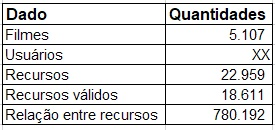
\includegraphics[scale=0.8]{imagens/dataset.jpg}
	\caption{Contagem dos dados utilizados durante os testes.}
	\label{fig:dataset}
\end{figure}

Os dados dos filmes foram extraídos do projeto MovieLens\footnote{https://movielens.org}, que possibilita a expansão dos dados com o IMDB\footnote{https://imdb.com}, uma vez que o mesmo também provê identificadores para esse serviço de banco de dados de filmes. Quanto aos dados do usuário, são em sua maioria gerados pela interação com sistema, partindo do seu cadastro que pode ser realizado pela própria plataforma, ou através do login pelo Facebook\footnote{https://facebook.com}. Essa opção de login facilita a coleta de dados como email, nome e até preferência de filmes, desde que estejam cadastrados no sistema. Após o login o sistema coletará dados da preferência do usuário seja parcialmente vindos pelo Facebook ou através da seleção pela próprio sistema. Por fim o sistema gera recomendações para o usuário que são persistidas para posterior coleta das suas avaliações.

Para a montagem do perfil do usuário, com seus termos foi utilizado um cálculo dos "n melhores termos únicos", conforme abordado no \ref{cap:proposal}. Foi determinado que serão 15 termos escolhidos para a montagem do perfil do usuário. A quantidade de termos definida possui um impacto grande na performance do sistema, uma vez que a complexidade do algoritmo da comparação entre termos é de $O(nm)$ (considerando $n$ como constante tem-se $O(m)$), sendo $n$ a quantidade de termos do usuário e $m$ a quantidade de termos do filme. A figura \ref{fig:tempo_x_termos} demonstra um gráfico da quantidade de termos em relação ao tempo de processamento, considerando que todos os dados estão no \textit{cache}, ou seja, o melhor caso.

\begin{figure}
	\centering
	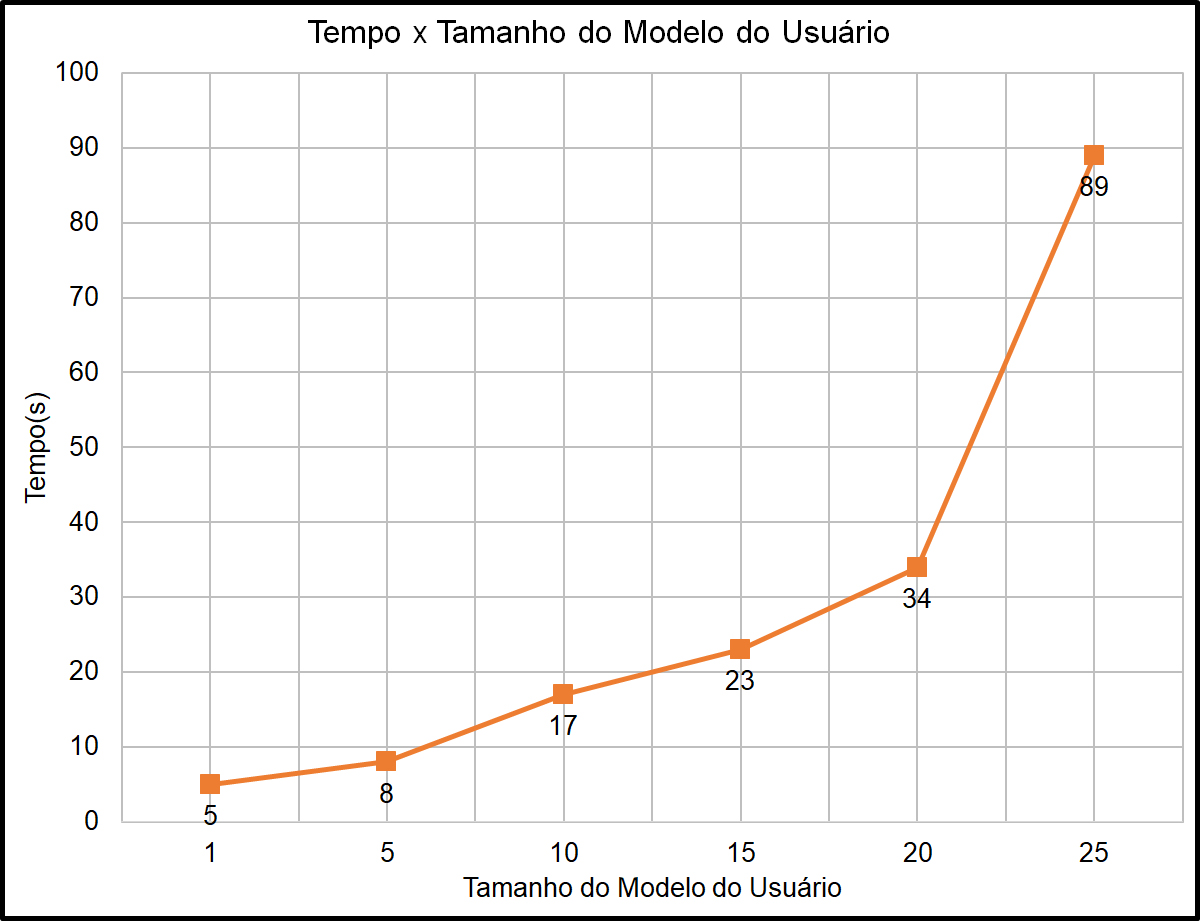
\includegraphics[scale=0.7]{imagens/tempo_x_termos.jpg}
	\caption{Gráfico da relação gráfico da quantidade de termos em relação ao tempo de processamento.}
	\label{fig:tempo_x_termos}
\end{figure}

Algo relevante para destacar quanto à relação entre recursos é de que a quantidade links diretos entre dois recursos maior que 0 é altamente rara, sendo apenas de 0,15\%. Já era esperado que a maioria dos recursos não tivesse propriedades diretamente conectadas entre si, devido a variedade de comparações indiscriminada entre termos do usuário e termos dos filmes. Isso resulta em tabela de dados altamente esparsa em relação ao cálculo a participação direta na fórmula \ac{RLWS}. A proporção de relacionamentos indiretos maiores que 0 em relação ao total é de 10,6\%. O quadro da figura \ref{fig:lod_cache_stats} apresenta outros resultados sobre os recursos, note que recursos redirecionados tratam-se de recursos relacionados que possuem a propriedade \textit{dbo:wikiPageRedirects}.

\begin{figure}
	\centering
	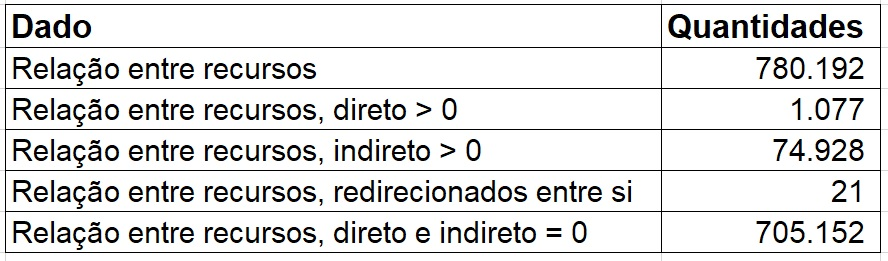
\includegraphics[scale=0.5]{imagens/lod_cache_stats.jpg}
	\caption{Tabela de dados com estatísticas das relações entre recursos.}
	\label{fig:lod_cache_stats}
\end{figure}

\section{Métricas de avaliação}

O estudo da avaliação de \ac{SR} é importante para entender sua eficácia e seus algoritmos envolvidos, uma vez que uma análise incorreta pode levar subestimação ou superestimação da sua real precisão, como aponta \cite{Aggarwal2016:Evaluation}. Sendo assim, recomendadores podem ser avaliados tanto usando métodos denominados como \textit{online} ou \textit{offline}. Num sistema \textit{online} as opiniões e reações dos usuários são consideradas e medidas de acordo com as recomendações apresentadas, sendo a participação real crucial para a compreensão dos resultados. Contudo, como a avaliação desse método requer a participação do usuário, o que nem sempre é viável, também existe o método \textit{offline}, onde um conjunto de diferentes tipos de dados históricos dos usuários são utilizados \citep{Herlocker:1999}.

Existem diversas métricas que são usadas tanto em avaliações \textit{online} e \textit{offline}, mas as mais comuns são as de \textit{accuracy}, embora existam outras como \textit{user coverage}, \textit{novelty}, \textit{trust} \citep{Jannach:2010}. Para este trabalho foi utilizada uma avaliação \textit{online} utilizando métodos de precisão para avaliar as classificações da recomendações, como \textit{Precision} e \textit{Recall}.

\subsection{Precision}

Avaliando recomendações com métodos \textit{offline} apenas utilizando dados históricos da preferência do usuário, somente pode informar daqueles itens que foram de conhecimento do usuário, portando todos os outros itens serão considerados como avaliações negativas que o usuário não tem interesse, podendo levando à falso positivos. Por outro lado, avaliando com usuários reais, esses podem julgar todos os itens recomendados, podendo de fato definir se a predição foi correta ou não. Com a avaliação do usuário é possível construir uma tabela de classificação conforme a figura \ref{fig:truth_table} \citep{Jannach:2010}, onde há cruzamento entre o que o recomendador apresentou e o que usuário avaliou. Se um item foi apresentado na recomendação e o usuário tenha gostado, avaliado como relevante, tem-se um caso de predição correta, ou \textit{true positive}. Outro resultado positivo, trata-se de quando o usuário não tenha gostado e o recomendador omitiu o resultado, ou seja uma omissão correta ou \textit{true negative}. Assim os resultados positivos estão na diagonal da esquerda para direita da tabela, e os resultados não desejados e negativos estão na outra diagonal. 

\begin{figure}
	\centering
	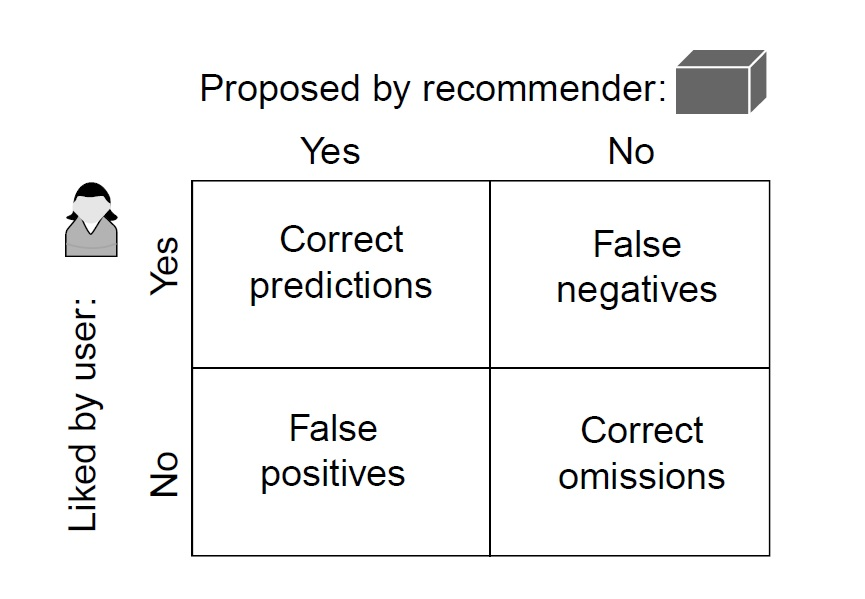
\includegraphics[scale=0.4]{imagens/truth_table.jpg}
	\caption{Tabela de tipos de erros retirada de \cite{Jannach:2010}.}
	\label{fig:truth_table}
\end{figure}

Considerando e classificando os resultados dessa forma binária, em positivos e negativos, defini-se \textit{precision}, precisão ou confiança, como sendo a fração resultados previstos e avaliados pelo usuário como positivos, ou seja, os \textit{true positive}, em relação a quantidade de todos os itens recomendados \citep{Powers_2008}. A fórmula \ref{eq:precision} demonstra o cálculo da precisão $P$, onde $tp$ trata-se da quantidade de itens \textit{true positive} e $fp$ como \textit{false positive}.

\begin{equation}
	P = \frac{tp}{tp + fp}
\label{eq:precision}
\end{equation}

Como a quantidade de resultados pode ser muito grande para calcular a precisão, e até para que o próprio usuário o faça, por extensão também defini-se como $P@k$, como sendo a precisão até $k$ primeiros resultados retornados pelo recomendador \citep{Aggarwal2016:Evaluation}.

\subsection{Recall}

Outra métrica de precisão utilizando classificações binárias, é o \textit{recall} que trata-se da proporção de resultados \textit{true positive} em relação ao total possível resultados positivos reais avaliados pelo usuário \citep{Powers_2008}. O valores irão progredir de 0 a 1 sempre, sendo o valor 1 atribuído para todos os elementos a partir (inclusive) do último item previsto como \textit{true positive}. O objetivo além de verificar quais os itens mais relevantes, é constatar o quão melhor eles se posicionam na ordem dos retornados, sendo o ideal que mais itens como \textit{true positive} estejam nos primeiros resultados \citep{Jannach:2010}. A fórmula \ref{eq:recall} demonstra o cálculo do \textit{recall} $R$, onde $tp$ trata-se da quantidade de itens \textit{true positive} e $fn$ como \textit{false negative}.

\begin{equation}
	R = \frac{tp}{tp + fn}
\label{eq:recall}
\end{equation}

Também por extensão podemos calcular $R@k$ como sendo o \textit{recall} até os $k$ primeiros resultados. Assim, primeiro obtém-se o total de itens relevantes até $k$ para ser utilizado como denominador da equação do original do \textit{recall}.

\subsection{Mean Average Precision (MAP)}

Outra métrica de precisão trata-se da \ac{MAP}, que busca estipular um único valor de precisão em relação ao conjunto de avaliações de múltiplos usuários \citep{Manning:2008}. A fórmula \ref{eq:map} demonstra o cálculo, onde $AveP(n)$ trata-se da média das precisões do $n$ ésimo usuário, e $N$ a quantidade de usuários que realizaram a avaliação.

\begin{equation}
	MAP = \frac{\sum_{n=1}^{N}AveP(n)}{N}
\label{eq:map}
\end{equation}

\section{Resultados}

Antes de apresentar os resultados das recomendações com as avaliações dos usuários, é importante verificar algumas premissas e comportamentos da própria fórmula de similaridade, \ac{RLWS}. Inicialmente o esperado que recursos que sejam intuitivamente próximos, ou provavelmente tenha diversas relações entre si,  como \textit{Earth} e \textit{Moon}, tenham maior similaridade do que \textit{Earth} e \textit{Table}. E de fato, mesmo nos dois extremos de pesos, seja priorizando as ligações diretas ou indiretas, existe uma diferença considerável quando termos estão intuitivamente mais próximos do que aqueles que provavelmente não terão relacionamentos em comum, conforme mostra figura da tabela de amostra de comparações \ref{fig:rlws_results}. Note que \textit{RLWS(0,8/0,2)} refere-se ao uso dos pesos como sendo 0,8 para links diretos e 0,2 para indiretos.

É importante ressaltar que mesmo para termos que estejam aparentemente mais distantes, como \textit{Selena\_Gomez} e \textit{Ariana\_Grande}, por se tratarem de "coisas" que não são imediatamente próximas, ainda possuem uma alta similaridade, devido as conexões que ambas as pessoas possuem quanto à música e aparições em temas de filmes, programas etc. Já quando compara-se \textit{Selena\_Gomez} com \textit{Elon\_Musk}, mesmo sendo pessoas a segunda tem menos relacionamentos, o que também é intuitivamente esperado. Esse comportamento também é observado na comparação \textit{Johnny\_Cash} e \textit{June\_Carter\_Cash}, pois os dois foram casados e cantores. Outra observação importante é quanto aos termos \textit{Car} e \textit{Automobile} que possuem similaridade 1. Isso é devido que os dois possuem a propriedade \textit{dbo:wikiPageRedirect} conectado seus recursos, o que por regra entra na clausula da fórmula tendo valor 1. Esses redirecionamentos também ocorrem nos  termos \textit{Future} e \textit{Futuristic}, \textit{Power} e \textit{Powerful} entre outros.

Nota-se que intuitivamente os resultados das comparações fazem sentido tanto usando pesos que privilegiam links diretos ou indiretos, o que é vital para coerência no momento da comparação termo a termo. Outro fato importante é a consideração de itens que possuem redirecionamentos, ainda que sejam raros, mas para palavras como "Carro" e "Automóvel" é sensato dizer que são similares.

\begin{figure}
	\centering
	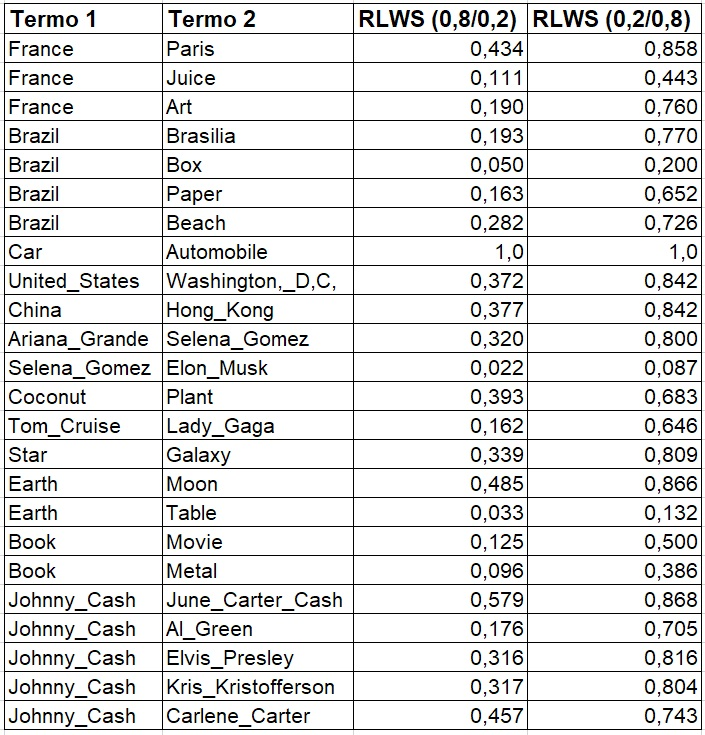
\includegraphics[scale=0.7]{imagens/rlws_results.jpg}
	\caption{Tabela de amostra de comparações entre termos usando \ac{RLWS}.}
	\label{fig:rlws_results}
\end{figure}

\subsection{Resultados das recomendações}

\section{Discussão dos resultados}
